\section{Diagrama P\&ID}

Um PI\&D (\emph{Piping and Instrumentation Diagram}) é um diagrama que coloca de forma bem compacta várias informações sobre os instrumentos ligados a um processo. Um exemplo pode ser visto na figura \ref{fig:exemploPID}. Neste diagrama, os instrumentos são representados por símbolos padrões, definidos pela norma ISA 51.

\begin{figure}[h]
  \centering
  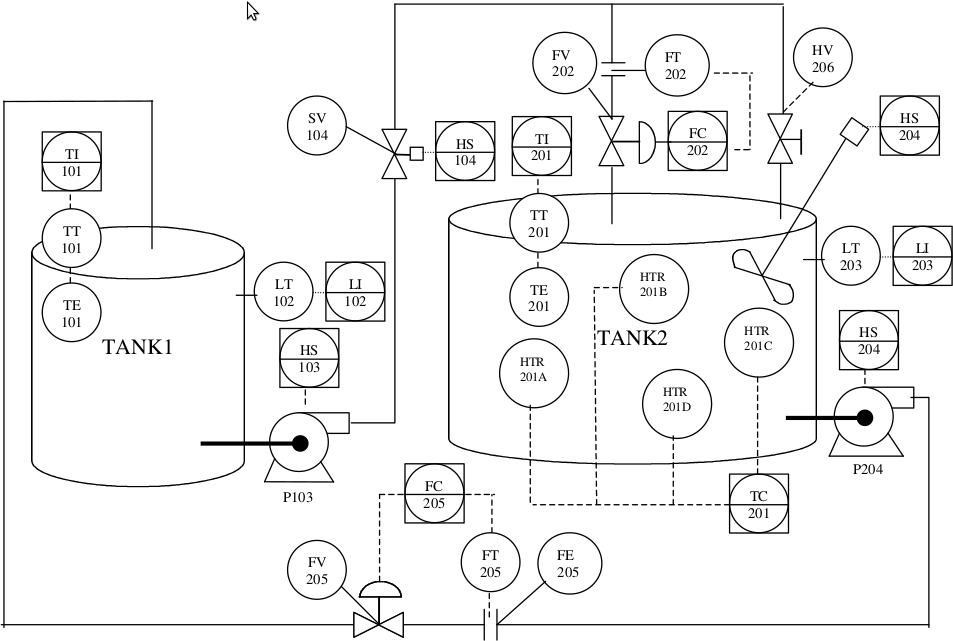
\includegraphics[width = 0.8\textwidth]{figuras/exemploPID}
  \caption{Exemplo de um diagrama P\&I.\label{fig:exemploPID}.}
\end{figure}

Cada instrumento é definido por um conjunto de letras e um número. A primeira letra indica que grandeza é relacionada àquele instrumento; a segunda letra em diante especifica a função daquele instrumento, com eventuais modificadores.
Exemplos:
\begin{description}
  \item[TRC --] \emph{Temperature Register and Controller}, controlador e registrador de temperatura.
  \item[PDIC --] \emph{Pressure (differential) Indicator and Controller}, controlador e indicador de pressão diferencial.
  \item[FAH --] \emph{High Flow Alarm}, alarme de vazão alta.
\end{description}

As funções mais comuns de um instrumento são:
\begin{description}
  \item[A -- Alarme.]
  \item[C -- Controlador.] Responsável por gerar o sinal de controle do atuador que afeta aquela variável.
  \item[I -- Indicador.] O instrumento permite ler o valor da variável nele.
  \item[T -- Transmissor.] O instrumento é um transdutor que gera um sinal padrão para outro instrumento.
\end{description}

O número é referente a malha de instrumentação. Normalmente é relacionado com a variável de processo que é controlada por aquele conjunto de instrumentos. Na própria figura \ref{fig:exemploPID}, na parte superior, o conjunto de instrumentos FT202, FC202 e FV202 fazem a malha de controle que mede (FT202), controla (FC202) e atua (FV202) na vazão de água do tanque 1 para o 2.

Vários instrumentos tem símbolos próprios, tais como bombas e válvulas. Outros instrumentos são representados por um símbolo (figura \ref{fig:simbolosISA}), contendo o código do mesmo, que indicam o que é o instrumento e onde ele está localizado.
\begin{figure}[h]
  \centering
  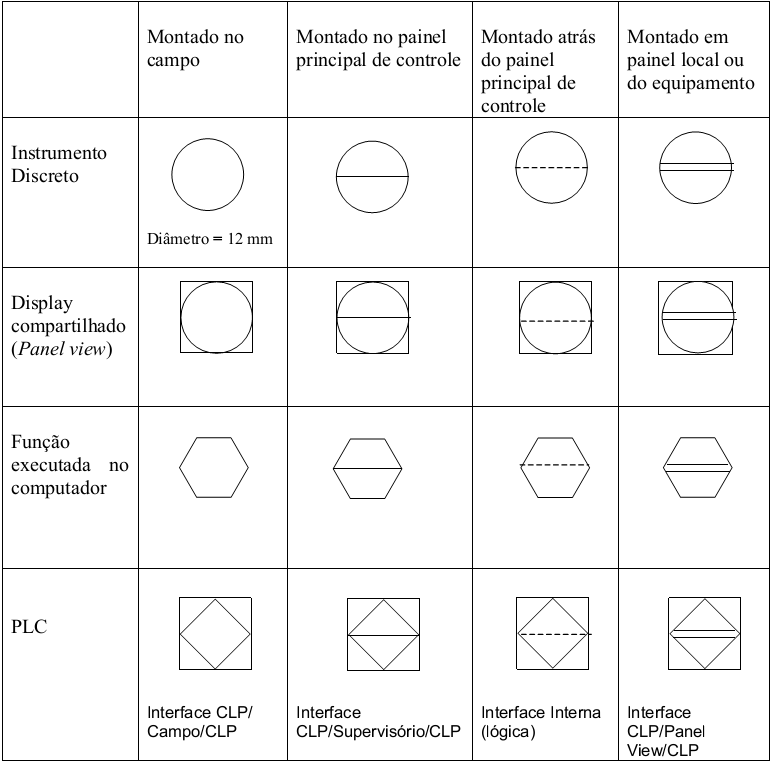
\includegraphics[width = 0.6\textwidth]{figuras/simbolosISA}
  \caption{Explicação dos símbolos dos instrumentos.\label{fig:simbolosISA}.}
\end{figure}

\subsection{Transmissão de dados}
\label{sub:TransmissaoDeDados}

As linhas que ligam os instrumentos são decoradas de acordo com a forma com que a informação passa de um instrumento para o outro, de acordo com a figura \ref{fig:linhasISA}.
\begin{figure}[h]
  \centering
  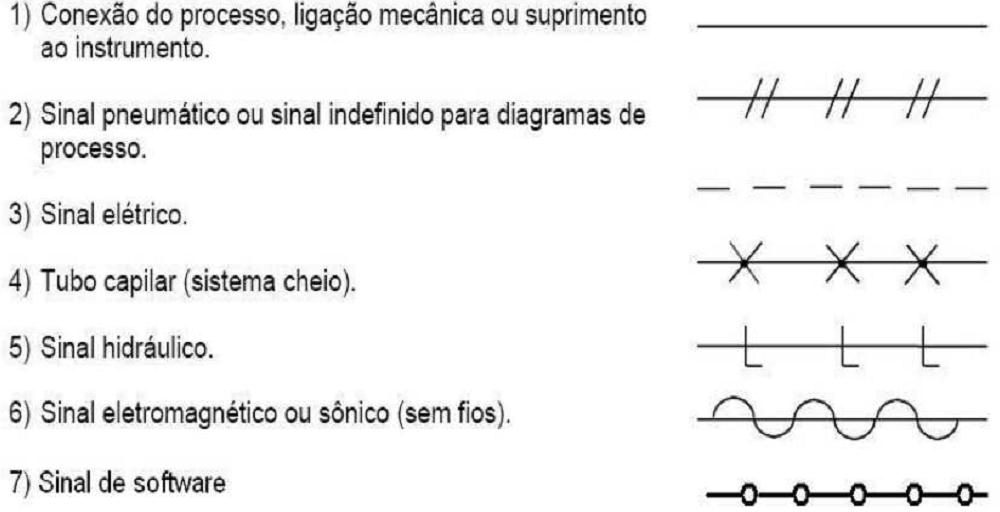
\includegraphics[width = 0.6\textwidth]{figuras/linhasISA}
  \caption{Explicação das linhas do diagrama P\&I.\label{fig:linhasISA}.}
\end{figure}

Sinais comuns são:
\begin{description}
  \item[Pneumáticos.] Usam gás comprimido na faixa de 20 a \SI{100}{\kilo\pascal}. É usado em áreas que se tenha risco de explosão. Tem limitação com a distância e é difícil de detectar vazamentos.

%  A razão de usar uma pressão mínima maior que a ambiente (aproximadamente \) é para facilitar a detecção de erros: Se o transmissor não funcionar a pressão vai cair para abaixo de \SI{20}{\kilo\pascal}
  \item[Hidráulico.] Usam óleo sobre pressão. São mais caros que sistemas pneumáticos porém são mais rápidos e podem até ser usados para acionar alguns equipamentos de grande porte.
  \item[Elétrico.] Usam um sinal de 4 a \SI{20}{mA} ou de 1 a \SI{5}{\volt} -- os receptores deste tipo de sinal tem internamente um resistor de \SI{250}{\ohm} em paralelo a sua entrada, o que permite que aceitem ambos tipos. A razão de usar um valor mínimo diferente de zero é para detectar uma falha de conexão que zere o sinal. O mais comum é o transmissor de corrente, pois são menos sujeitos a interferências.
  \item[Sinais digitais.] São sinais elétricos modulados de acordo com um protocolo de comunicação digital. São usados nos chamados sensores inteligentes e estão ficando cada vez mais comuns. Existem muito protocolos diferentes no mercado, com pouca compatibilidade entre eles.

  Dependendo do protocolo usado, podem ter um custo total menor que o elétrico analógico por redução de cabeamento. Além disto, a comunicação digital permite passar outras informações, tais como configurações, dados de calibração e diagnósticos.

  \item[Rádio.] Normalmente usam sinais digitais modulados em rádio frequência. São muito usados para longas distâncias e para equipamentos móveis. Interferência e problemas de segurança diminuem seu uso mais geral.
\end{description}
